%\documentclass[a4paper,12pt,oneside,openright,final]{memoir} %twocolumn,
\documentclass[a4paper,12pt,oneside,openright]{memoir}

\let\footruleskip\undefined
\usepackage[utf8]{inputenc}
\usepackage[english]{babel}
\usepackage{etex}
\usepackage{times}
\DisemulatePackage{setspace}
\usepackage{setspace}
\usepackage{amssymb}
\usepackage{amsfonts}
\usepackage{underscore} % allows the use of _ in text without escaping
% for making quotations
\usepackage{etoolbox}
\AtBeginEnvironment{quote}{\singlespacing\small}
\usepackage{csquotes}

\usepackage{verbatim}
\usepackage{enumitem}

\usepackage{graphicx}
\usepackage[printwatermark]{xwatermark}
% uncomment for watermarks
\newwatermark[allpages,color=gray!10,angle=45,scale=5,xpos=-15,ypos=30]{DRAFT}

\usepackage{alltt}
\usepackage{moreverb}
\usepackage{xcolor}
\definecolor{basiccolor}{HTML}{000000}%1435AD
\definecolor{highlight}{HTML}{FFB100}
\definecolor{greenlink}{HTML}{558b2f}
\definecolor{bluegraylink}{HTML}{455a64}
%for more info on hyperref package see http://en.wikibooks.org/wiki/LaTeX/Packages/Hyperref
\usepackage[colorlinks=true,linkcolor=bluegraylink,citecolor=magenta]{hyperref}
\usepackage{eso-pic}
\usepackage{transparent}
\setlength{\columnsep}{3em}

\usepackage[export]{adjustbox}%enables "right", "left" and "center" for images
\usepackage{wrapfig}
\usepackage{caption}
\usepackage{subcaption}
\usepackage{alltt}
\usepackage{moreverb}
% tikz related packages to provide scalable graphics
\usepackage{tikz}
\usetikzlibrary{calc,mindmap,backgrounds,positioning,arrows,shapes,shapes.multipart,shapes.arrows,shapes.misc,automata,petri,patterns,scopes,chains,matrix,decorations.pathmorphing,shadows,calc,trees}

\tikzset{
  treenode/.style = {shape=rectangle, rounded corners,
                     draw, align=center,
                     top color=white, bottom color=blue!20},
  root/.style     = {treenode, font=\Large, bottom color=red!30},
  env/.style      = {treenode, font=\ttfamily\normalsize},
  dummy/.style    = {circle,draw}
}


\usepackage{geometry}
\geometry{hmargin={15mm,15mm},vmargin={15mm,20mm}}

\usepackage[pages=some]{background}

\backgroundsetup{
  scale=1.2,
  angle=0,
  opacity=0.4,
  contents={
    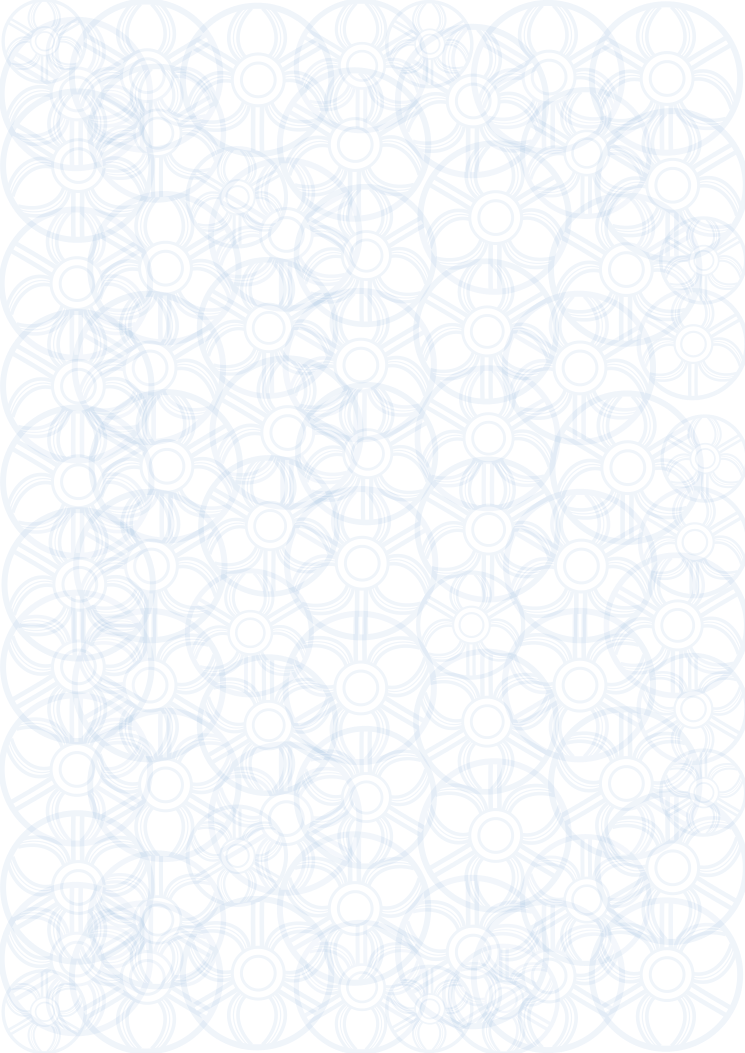
\includegraphics[width=1.1\paperwidth,height=1.1\paperheight, keepaspectratio]{images/00-background.png}}
}


%%%%%%%%%%%%% copyright %%%%%%%%%%%%%%
\usepackage{hyperxmp}
\hypersetup{
    pdftitle={Roadmap 2019},
    pdfsubject={Trident Genesis},
    pdfauthor={Fielden Management Services Pty. Ltd.},
    pdfcopyright={Copyright (C) 2019 by Fielden Management Services Pty. Ltd.  All rights reserved.}
}

\makepagestyle{fmsstyle}% Define 'fmsstyle' page style
  \makeevenfoot{fmsstyle}{\color{gray}Copyright \textcopyright\ 2019 by Fielden Management Services Pty. Ltd.  All rights reserved.}{}{\thepage}% Even page footer
  \makeoddfoot{fmsstyle}{\color{gray}Copyright \textcopyright\ 2019 by Fielden Management Services Pty. Ltd.  All rights reserved.}{}{\thepage}% Odd page footer
\pagestyle{fmsstyle}% Set page style to 'fmsstyle'

\usepackage[T1]{fontenc}
\usepackage{lmodern}
\usepackage{url}
\usepackage{pdfcolmk}
%% for dingbats
\usepackage{pifont}


\newcommand*{\titleTH}{\begingroup% T&H Typography
\raggedleft
\vspace*{\baselineskip}
{\Large ~}\\[0.167\textheight]
{\bfseries Trident Genesis}\\[\baselineskip]
{\textcolor{basiccolor}{\Huge Roadmap 2019}}\\[\baselineskip]
{\small Research \& Development}\par
\vfill
{\Large Fielden Management Services Pty Ltd}\par
\vspace*{1\baselineskip}
{\emph{Draft:} Aug 01, 2019}\par
\endgroup}

%%%%%%%%%%%%%%%%%%%%%%%%%%%%%%%%%
%%%%%%%%%%%%%%%%%%%%%%%%%%%%%%%%%
%%%%%%%%%%% Document %%%%%%%%%%%%
%%%%%%%%%%%%%%%%%%%%%%%%%%%%%%%%%
%%%%%%%%%%%%%%%%%%%%%%%%%%%%%%%%%
\begin{document}

\chapterstyle{article}
\pagestyle{fmsstyle}

\titleTH
\thispagestyle{empty}

\frontmatter
\doublespacing
\chapter{Preface}
\paragraph{Keywords:} \emph{Conceptual Modelling, Information Systems, Software Architecture, Software Engineering, Domain-Driven Design, Test-Driven Development.}
\vspace*{1em}

The purpose of this document is outline R\&D directions for advance the Trident Genesis platform.
There are 3 broad research categories, which are largely segregated from each other:

\begin{itemize}
    \item \textbf{Software Engineering}: modelling, automation, design and runtim tooling (verification, validation, visualisation), ;
    \item \textbf{User Interface and User Experience}: interaction with domain models, configurability, more advanced and smarter controls, notifications.
    \item \textbf{Integration}: GraphQL API.
\end{itemize}

\noindent And there are 3 broad categories that address cross-cutting concerns of the technology, which affect all of the above categories:

\begin{itemize}
    \item \textbf{Runtime Performance}: snappier UI, faster load times, optimised data queries and caching, more compile time optimisation.
    \item \textbf{Security}: improvements to application security, more refined read access control to entity properties, authenitcation and authorisation of 3rd party integrators.
    \item \textbf{Capabilities}: offline mode, scalability, async request process, task scheduling, auditing, even sourcing.
\end{itemize}


\section{Objectives}



\begin{spacing}{1}
\tableofcontents
\end{spacing}

\mainmatter
\chapter{Java VM and Language}
At the moment we utilise Java~8 for developing the core of the server-side technology.
The next big jump of Java after version~8 was version~9 from both the programming language and JVM perspective.
All subsequent versions of Java, including the latest version~12, are incremental improvements of version~9.
In this document we shall refer to all these newer Java versions as ``Java~9''.

This release direction should explore the advantages that Java~9 offers to 
\begin{itemize}
  \item Migration to  Java 9 and above.
  \item Research on using Java 9 modules to improve segregation of bounded contexts.
  \item Research OpenJDK projects such as Valhalla to see how they can be leveraged to improve modelling and runtime performance.
\end{itemize}

\chapter{Object-relational mapping}

The Hibernate ORM solution served us relatively well thus far.
However, fundamentally it stand in a way of a more performant and lean ORM solution that would take advantage of the model metadata used by TG applications.

\chapter{Code generation and static model verification}

Java requires for properties to have \texttt{setter} and \texttt{getter} methods.
By design, TG entities don't need and should not have any logic in such methods.
Therefore, there is no need to these methods even exist in the code source if they could be present in the binary class representation. 
Project \href{https://projectlombok.org/}{Lobmok} is an excellent example of how a lot of boilerplate code could be eliminated.

\href{http://hannesdorfmann.com/annotation-processing/annotationprocessing101}{Annotation Processing 101}


\end{document}

